\documentclass[a4paper, 12pt]{article}

%%% SST LAB PROTOCOLL PREAMBLE
%%% 2019
%%%%%%%%%%%%%%%%%%%%%%%%%%%%%%%


%%% PACKAGES
%%%%%%%%%%%%%%%%%%%%%%%%%%%

\usepackage[ngerman]{babel}

\usepackage[utf8]{inputenc}
\usepackage{amsmath}
\usepackage{pgfplots}
\usepackage{tikz}
\usepackage[many]{tcolorbox}
\usepackage{graphicx}
\graphicspath{ {./graphics/} }
\usepackage{pdfpages}
\usepackage{dashrule}
\usepackage{float}
\usepackage{siunitx}
\usepackage{trfsigns}
\usepackage{booktabs}
\usepackage[european]{circuitikz}
\usepackage{tcolorbox}

%%% DOCUMENT GEOMETRY
%%%%%%%%%%%%%%%%%%%%%%%%%%%

\usepackage{geometry}
\geometry{
 a4paper,
 total={0.6180339887498948\paperwidth,0.6180339887498948\paperheight},
 top = 0.1458980337503154\paperheight,
 bottom = 0.1458980337503154\paperheight
 }
\setlength{\jot}{0.013155617496424828\paperheight}
\linespread{1.1458980337503154}

\setlength{\parskip}{0.013155617496424828\paperheight} % paragraph spacing


%%% COLORS
%%%%%%%%%%%%%%%%%%%%%%%%%%%

\definecolor{red1}{HTML}{f38181}
\definecolor{yellow1}{HTML}{fce38a}
\definecolor{green1}{HTML}{95e1d3}
\definecolor{blue1}{HTML}{66bfbf}
\definecolor{hsblue}{HTML}{00b1db}
\definecolor{hsgrey}{HTML}{afafaf}

%%% CONSTANTS
%%%%%%%%%%%%%%%%%%%%%%%%%%%
\newlength{\smallvert}
\setlength{\smallvert}{0.0131556\paperheight}


%%% COMMANDS
%%%%%%%%%%%%%%%%%%%%%%%%%%%

% differential d
\newcommand*\dif{\mathop{}\!\mathrm{d}}

% horizontal line
\newcommand{\holine}[1]{
  	\begin{center}
	  	\noindent{\color{hsgrey}\hdashrule[0ex]{#1}{1pt}{3mm}}\\%[0.0131556\paperheight]
  	\end{center}
}

% mini section
\newcommand{\minisec}[1]{ \noindent\underline{\textit {#1} } \\}

% quick function plot
\newcommand{\plotfun}[3]{
  \vspace{0.021286\paperheight}
  \begin{center}
    \begin{tikzpicture}
      \begin{axis}[
        axis x line=center,
        axis y line=center,
        ]
        \addplot[draw=red1][domain=#2:#3]{#1};
      \end{axis}
    \end{tikzpicture}
  \end{center}
}

% box for notes
\newcommand{\notebox}[1]{

\tcbset{colback=white,colframe=green1!100!black,title=Note!,width=0.618\paperwidth,arc=0pt}

 \begin{center}
  \begin{tcolorbox}[]
   #1 
  \end{tcolorbox}
 
 \end{center} 
 
}

% box for equation
\newcommand{\eqbox}[2]{
	
	\tcbset{colback=white,colframe=green1!100!black,title=,width=#2,arc=0pt}
	
	\begin{center}
		\begin{tcolorbox}[ams align*]
				#1
		\end{tcolorbox}
		
	\end{center} 
	
}
% END OF PREAMBLE

\renewcommand{\thesubsection}{\thesection.\alph{subsection}}
%%%%%%%%%%%%%%%%%%%%%%%%%%%%%%%%%%%%%

\begin{document}

% 1
%%%%%%%%%%%%%%%%%%%%%%%%%%%%%%%%%%%%%
  % 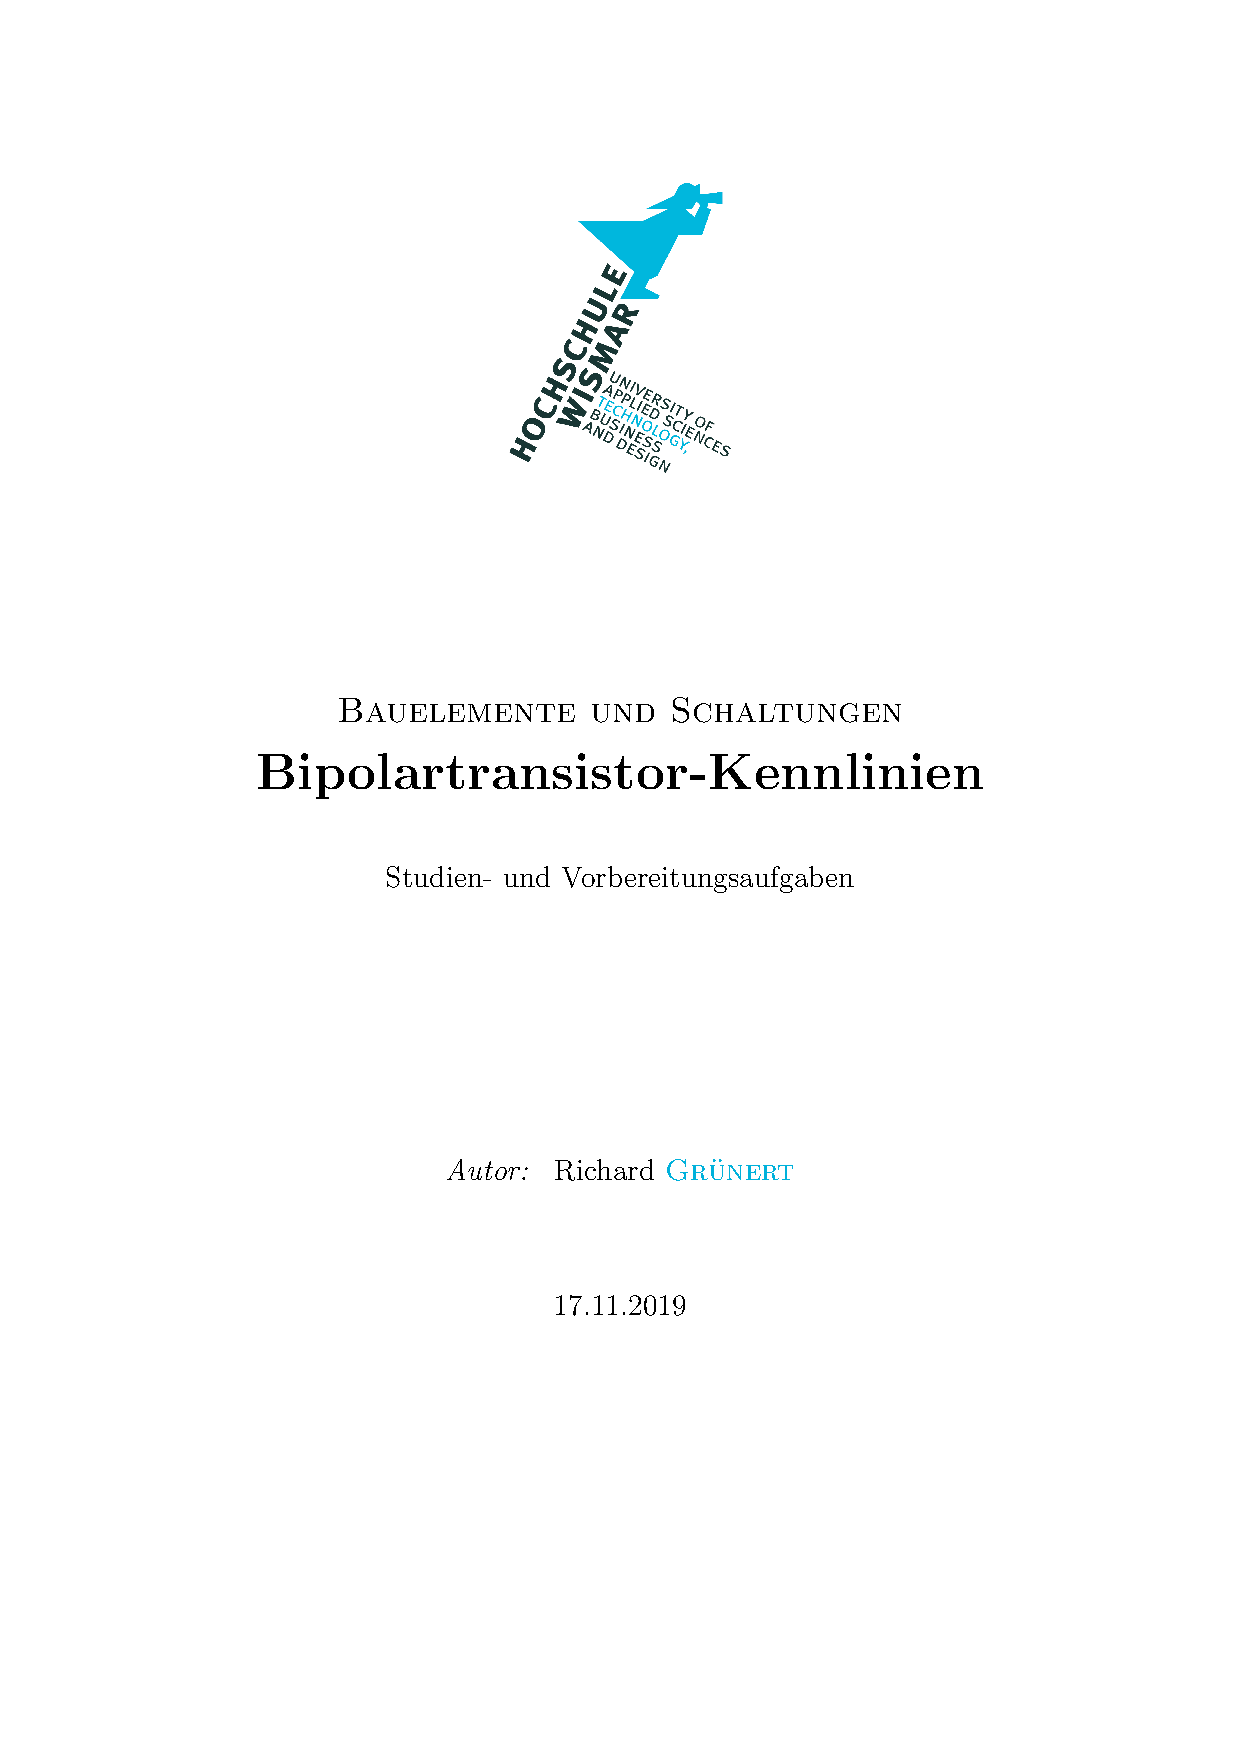
\includepdf{./titlepage/titlepage1.pdf}
  % \clearpage
  % \setcounter{page}{1}
%%%%%%%%%%%%%%%%%%%%%%%%%%%%%%%%%%%%%

 \section{Aufgabe 1} 
 \subsection{RZ-Bandbreite}
 Bei der Return-to-Zero (RZ) Übertragung entspricht die Bitrate der Bandbreite
 \[B_{RZ} = BR = 2\, \si{\mega\hertz}\]

 Die RZ-Übertragung besitzt gegenüber der der NRZ-Übertragung die doppelte
 Bandbreite, da bei gleicher Zeit für ein Bit $\tau_b$, d.h. bei gleicher
 Bitrate, eine Rechteckfolge mit halbierter Periodendauer/doppelter Frequenz
entsteht.
 \begin{figure}[H]
 \begin{center}
   \resizebox{0.382\textwidth}{!}{\input{rz.pdf_tex}}
 \end{center}
 \end{figure}


 % Bei der NRZ-Übertragung ist die Näherung der Bandbreite gegeben durch die
 % Breite des Spektrums bis zum ersten Nulldurchgang bei $1/{\tau_b}$. Die Bitrate
 % ist $BR = 1/{\tau_b}$

 \subsection{Bandwidth / Rise Time}
 Der Zusammenhang zwischen Signalanstiegszeit (\emph{rise time}) und Bandbreite ist gegeben durch
 \[B = \frac{0.35}{t_{\mathrm{rise}}} = \frac{0.35}{1 \, \si{\nano\second}} =
   350 \, \si{\mega\hertz}\]


\subsection{Netzwerkanalysator}
Der Netzwerkanalysator hat einen nach außen geführten internen Wobbel-Generator,
welcher als Eingangssignalquelle für das DUT verwendet wird. Der Ausgang des
DUTs wird an den Eingang des NWAs geführt.

Da dem NWA die momentane Testfrequenz und Testamplitude bekannt ist, kann er die
Amplitude messen und damit die Dämpfung bzw. Verstärkung bei dieser Frequenz, die durch den Frequenzgang des DUTs entsteht, als Punkt in
einem Graph darstellen.

Die Auflösung hängt dabei vom Abstand der Durchlaufenen Frequenzen ab.

\subsection{Impulsmessverfahren zur Bandbreitenbestimmung}
Das Impulsmessverfahren verwendet einen Impulgenerator zur Erzeugung eines
möglichst schmalen Impulses. Die Idee dahinter ist, einem \emph{Dirac-Impuls} so
nahe wie möglich zu kommen, da dieser theoretisch alle Frequenzen gleichzeitig
mit gleicher Amplitude enthält.

Der Impuls wird auf das DUT gegeben. Da sich das Ausgangs-Zeitsignal als \emph{Faltung}
des Eingangssignals mit der Impulsantwort (Gewichtsfunktion) des DUTs ergibt, entsteht im
Frequenzbereich die \emph{Multiplikation} des Frequenzganges des DUTs mit dem
über alle Frequenzen konstanten Frequenzgang des Testimpulses. Der Frequenzgang
am Ausgang entspricht demnach dem Frequenzgang des DUTs (skaliert mit der
Amplitude/Impulsdauer des Testimpulses). Über eine FFT kann das resultierende gemessene Zeitsignal am Oszilloskop oder am Computer in den Frequenzbereich
transformiert werden.

\subsection{(negative) Einflussgrößen beim Impulsmessverfahren}
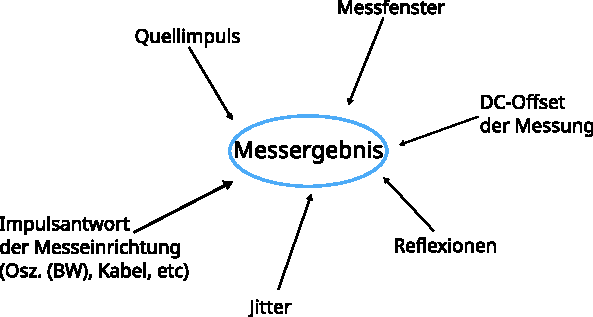
\includegraphics[width=\textwidth]{einflussdiag}

\subsubsection{Quellimpuls}
Ist der Quellimpuls zeitlich zu lang, ist seine obere Grenzfrequenz
möglicherweise kleiner als die des DUTs. Dadurch würde der Quellimpuls den
Frequenzgang des DUTs bei höheren Frequenzen negativ beeinflussen und somit die
Messung verfälschen (Multiplikation beider Frequenzgänge im FB).

Eine mögliche Lösung:
\[H_{\mathrm{meas}}(f) = H_{\mathrm{impuls}}(f) \cdot H_{\textrm{DUT}}(f)\]
\notebox{
\[\rightarrow H_{\mathrm{DUT}}(f) = \frac{H_{\mathrm{meas}}(f)}{H_{\mathrm{impuls}}(f)}\]

bzw. logarithmisch:
\[H_{\textrm{DUT}_{dB}} = H_{\mathrm{impuls}_{dB}} - H_{\mathrm{meas}_{dB}}\]
}

Kennt man also die Impulsantwort kann man mit diesem Wissen den (\glqq richtigen\grqq) Frequenzgang des
DUTs aus der Messung bestimmen.

Oder halt Entfaltung (Dekonvolution).
\href{https://de.wikipedia.org/wiki/Dekonvolution}{Wikipedia}

\subsubsection{Messfenster}

\subsubsection{DC-Offset}

\subsubsection{Reflexionen}

\subsubsection{Jitter}

\subsubsection{Messeinrichtung}

\subsection{Sampling-Oszilloskop}

\subsubsection{Vorteile}
\subsubsection{Nachteile}
 
\end{document}
